%%%%%%%%%%%%
%
% $Autor: Wings $
% $Datum: 2019-03-05 08:03:15Z $
% $Pfad: ArduinoIDEWeb.tex $
% $Version: 4250 $
% !TeX spellcheck = en_GB/de_DE
% !TeX encoding = utf8
% !TeX root = filename 
% !TeX TXS-program:bibliography = txs:///biber
%
%%%%%%%%%%%%


\chapter{Arduino Web Editor}


\section{Using the Arduino Web Editor}


The Arduino Web Editor allows you to write code and upload sketches to any official Arduino board directly from your web browser (Chrome, Firefox, Safari and Edge).

This IDE (Integrated Development Environment) is part of Arduino Create, an online platform that enables developers to write code, access tutorials, configure boards, and share projects. Designed to provide users with a continuous workflow, Arduino Create connects the dots between each part of a developer's journey from inspiration to implementation. Meaning, you now have the ability to manage every aspect of your project right from a single dashboard.

The Arduino Web Editor is hosted online, therefore it is always be up-to-date with the latest features and support for new boards.This IDE lets you write code and save it to the Cloud, always backing it up and making it accessible from any device. It automatically recognizes any Arduino board connected to your PC, and configures itself accordingly.

All you need to get started is an Arduino account. The following steps can guide you to start using the Arduino Web Editor: \cite{arduinoWebEditor:2024}

\begin{itemize}
    \item \textbf{Using the online IDE}
\end{itemize}

After logging in, you are ready to start using the Arduino Web Editor. The web app is divided into three main columns. ~\ref{web-editor}

\begin{figure}
    \begin{center}
        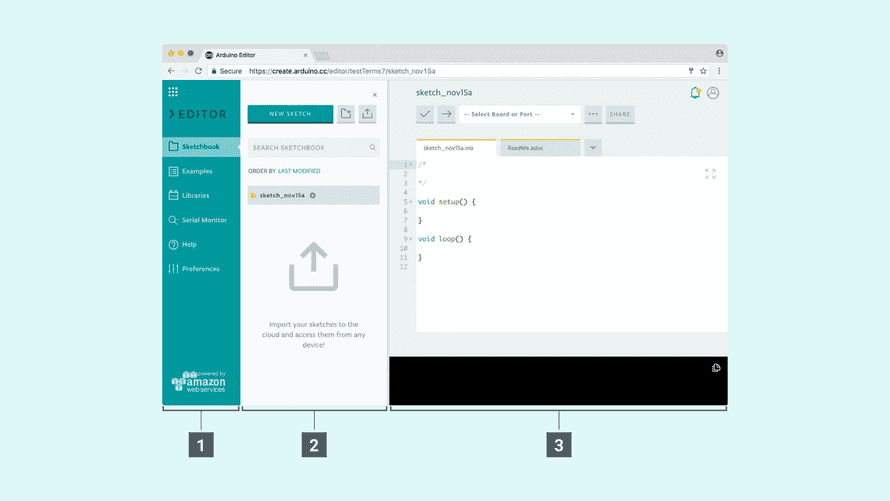
\includegraphics[width=0.7\linewidth]{Arduino/ArdiunoIDE2/web-editor.png}
        \caption{web-editor}
        \label{web-editor}
    \end{center}
\end{figure}

The Arduino Web Editor’s interface is as follows:

1. The first column lets you navigate between:

\textbf{Your Sketchbook}: a collection of all your sketches (a sketch is a program you upload on your board). \newline
\textbf{Examples}: read-only sketches that demonstrate all the basic Arduino commands (built-in tab), and the behavior of your libraries (from the libraries tab). \newline
\textbf{Libraries}: packages that can be included to your sketch to provide extra functionalities. \newline
\textbf{Serial monitor}: a feature that enables you to monitor, receive and send data to and from your board via the USB cable. \newline
\textbf{Help}: helpful links and a glossary about Arduino terms. \newline
\textbf{Preferences}: options to customize the look and behavior of your editor, such as text size and color theme.
\newline

2. The second column views the content of the chosen option.

3. The third column, the code area, is the one you will use the most. Here, you can write code, verify it and upload it to your boards, save your sketches on the Cloud, and share them with anyone you want.

\textbf{Now that you are all set up, let’s try to make your board blink}!

1. Connect your Arduino or Genuino board to your computer. Boards and serial ports are auto-discovered and selectable in a single dropdown. Pick the Arduino/Genuino board you want to upload to from the list at the top of the third column.

2. Let’s try an example: Choose Examples on the menu on the left (first column), then Basic and Blink. The Blink sketch is now displayed in the code area. 

\begin{figure}
    \begin{center}
        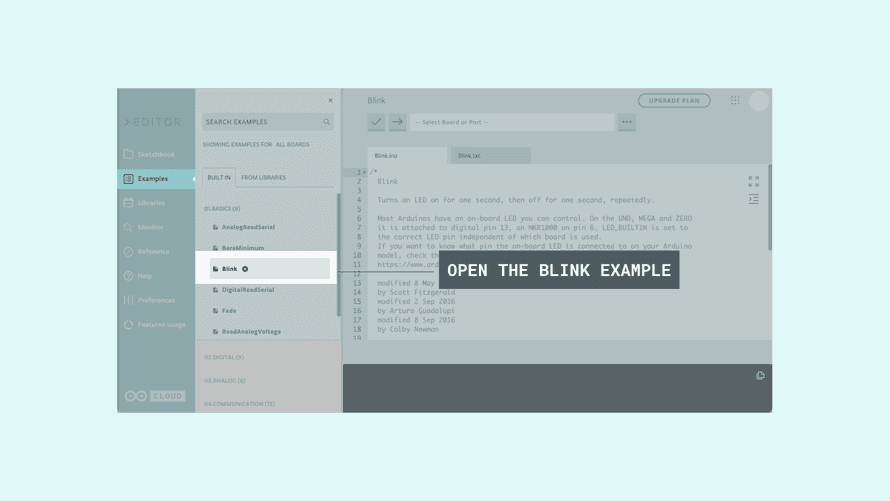
\includegraphics[width=0.7\linewidth]{Arduino/ArdiunoIDE2/finding-an-example.png}
        \caption{finding-an-example}
        \label{finding-an-example}
    \end{center}
\end{figure}

3. To upload it to your board, press the "Upload" button near the dropdown menu. While the code is verifying and uploading, a "BUSY" label replaces the upload button. If the upload is successful, the message "Success: done uploading" will appear in the bottom output area.

4. Once the upload is complete, you should see on your board the yellow LED with an L next to it start blinking. You can adjust the speed of blinking by changing the delay number in the parenthesis to 100, and upload the Blink sketch again. Now the LED should blink much faster. ~\ref{finding-an-example}

\section{Get to know Arduino Libraries}

The process of setting up libraries on the online IDE (Arduino Cloud Editor) is quite similar to the offline one:

1. Login to the Arduino Cloud.

2. Create or open a sketch.

3. Open the "Libraries" tab from the left menu, and search for libraries. The list displays read-only libraries, authored and maintained by the Arduino team and its partners.

4. When you find the library, you can add it to your sketch by selecting the "Include" button. You can also see the related examples, and select a specific version, if available.

5. If you can't find a specific library on the list, you can search every existing library through the search bar. You also have the option to add them to your favorites list by clicking on the star next to the library you want. Once you star a library, you can view it under the "favorites" tab and use its examples (if available).

\section{Data Security}

\begin{itemize}
    \item{Encryption}
    The web version of Arduino IDE should employ strong encryption protocols to ensure that data transmitted between the user's browser and the server is encrypted. This prevents unauthorized parties from intercepting and accessing sensitive information.
    
    \item{Secure Storage}
    User data, including login credentials and project files, should be securely stored on the server. This involves using robust encryption methods to protect data at rest, safeguarding it from unauthorized access or tampering.
\end{itemize}

\subsection{Authentication and Authorization}

\begin{itemize}
    \item{Strong Password Policies}
    Users should be encouraged to create strong, unique passwords for their accounts. The 	platform should enforce password complexity requirements and offer features like multi-factor authentication for added security.
    
    \item{Role-Based Access Control}
    The platform should implement role-based access control mechanisms to ensure that users only have access to the resources and features that are necessary for their roles. This helps prevent unauthorized access to sensitive functionality or data.
    
\end{itemize}

\subsection{Secure Code Execution}

\begin{itemize}
    \item {Sandboxing}
    The platform should execute user-uploaded code within a sandboxed environment to prevent it from accessing system resources or executing malicious commands. Sandboxing restricts the code's capabilities to ensure that it operates within predefined boundaries.
    \item {Code Validation}
    Before executing user code, the platform should perform thorough validation to detect and prevent common vulnerabilities such as code injection attacks or buffer overflows. This helps ensure that only safe and well-formed code is executed.
\end{itemize}

\subsection{Protection Against Malware}

\begin{itemize}
    \item {Code Scanning}
    The platform should employ code scanning techniques to detect and block malicious code uploaded by users. This involves analyzing code for known malware signatures, suspicious patterns, or potentially harmful behaviors.
    \item {Antivirus Integration}
    Integration with antivirus solutions can provide an additional layer of protection against malware. The platform can scan uploaded files for viruses or other malicious content before allowing them to be executed.
\end{itemize}


\subsection{Privacy Policies}

\begin{itemize}
    \item{Transparency}
    The platform should maintain transparent privacy policies that clearly outline how user data is collected, stored, and used. This includes information about data retention periods, third-party data sharing practices, and user consent requirements.
    \item {User Consent}
    Users should be informed about the platform's privacy practices and provide explicit consent for the collection and processing of their personal data. They should also have the ability to review and modify their privacy settings as needed.
\end{itemize}

\subsection{Regular Updates and Maintenance}

\begin{itemize}
    \item {Patch Management}
    The platform should have robust patch management processes in place to promptly address security vulnerabilities as they are discovered. This involves regularly updating software components, libraries, and dependencies to mitigate known security risks.
    \item {Security Audits}
    Regular security audits and penetration testing can help identify and remediate potential security 	weaknesses in the platform. These audits should be conducted by qualified security professionals to ensure thorough coverage and accuracy.
\end{itemize}

\subsection{User Awareness}

\begin{itemize}
    \item {Security Education}
    The platform should provide educational resources and guidance on secure coding practices, such as avoiding common vulnerabilities like cross-site scripting (XSS), SQL injection, and insecure direct object references.
    \item {Security Alerts}
    Users should receive timely alerts and notifications about security-related issues, such as suspicious login attempts, unauthorized access to their accounts, or security updates affecting their projects.
\end{itemize}









